% =============================================================================
\section{NPC Visitors}\label{sec:npc}
\subsection{Visitor life cycle}
Visitors appear only inside a car at the far end of the road. A new car comes every 8--18 s when a parking spot is
free and the road entrance is clear; at most six visitors are active at once. Every visitor is a state machine
(\Cref{fig:visitorsm}).
\begin{figure}[H]
\centering
\begin{tikzpicture}[node distance=0.9cm and 1.0cm]
\node[state] (a) {DRIVE IN\\road path};
\node[state,right=of a] (b) {WAIT\\for lot};
\node[state,right=of b] (c) {PARKING\\B\'ezier};
\node[state,right=of c] (d) {EXIT CAR\\door opens};
\node[state=yellow!15,below=0.9cm of d] (e) {INSIDE\\walk + activities};
\node[state,left=of e] (f) {ENTER CAR};
\node[state,left=of f] (g) {WAIT\\(clear aisle)};
\node[state,left=of g] (h) {UNPARK\\reverse};
\node[state,below=0.9cm of h] (i) {DRIVE OUT\\then removed};
\draw[arr] (a)--(b); \draw[arr] (b)--node[lbl,above=4pt]{token}(c); \draw[arr] (c)--(d); \draw[arr] (d)--(e);
\draw[arr] (e)--(f); \draw[arr] (f)--(g); \draw[arr] (g)--node[lbl,above=4pt]{token}(h); \draw[arr] (h)--(i);
\end{tikzpicture}
\caption{Visitor state machine.}\label{fig:visitorsm}
\end{figure}

\subsection{Driving and parking}
A car follows a \emph{path}, a list of points with the running length $s$. The position is interpolated at $s$ and the
heading is the direction of the current segment. The road path samples $z_{road}(x)$ every 3 m. Parking uses a cubic
Bézier curve
\[
\mathbf{B}(t) = (1-t)^3\mathbf{P}_0 + 3(1-t)^2t\,\mathbf{P}_1 + 3(1-t)t^2\,\mathbf{P}_2 + t^3\mathbf{P}_3,\qquad t\in[0,1],
\]
with $\mathbf{P}_0=(x_s+5,16)$ and $\mathbf{P}_1=(x_s+2.2,16)$ on the aisle and $\mathbf{P}_2=(x_s,z_s\pm2.8)$ and
$\mathbf{P}_3=(x_s,z_s)$ in the spot. Since $\mathbf{B}'(0)=3(\mathbf{P}_1-\mathbf{P}_0)$ and $\mathbf{B}'(1)=3(\mathbf{P}_3-\mathbf{P}_2)$,
the curve leaves along the aisle and enters straight into the spot. Leaving uses a second curve driven in
\emph{reverse} (heading = direction of motion $+180^\circ$, reverse lights on), then the car drives forward to the west end
of the road.
\begin{figure}[H]
\centering
\begin{tikzpicture}[x=0.6cm,y=-0.6cm,pt/.style={circle,fill,inner sep=1.4pt},lab/.style={font=\scriptsize}]
\fill[gray!30] (-2,8.6) rectangle (13,18.5);
\foreach \x in {0,6} {\draw[white,line width=1.5pt] (\x,8.9)--(\x,13.5);}
\draw[white,dashed] (-2,16)--(13,16);
\node[lab] at (3,9.5) {parking spot};
\draw[very thick,blue,-{Stealth[length=2.5mm]}] (8,16) .. controls (5.2,16) and (3,13.8) .. (3,11.2);
\draw[thick,red,dashed,-{Stealth[length=2.5mm]}] (3.25,11.2) .. controls (3.25,13.6) and (5.4,15.7) .. (8,15.7) -- (12.5,15.7);
\draw[gray] (8,16)--(5.2,16); \draw[gray] (3,13.8)--(3,11.2);
\node[pt,label={[lab]below:$P_0$}] at (8,16) {};
\node[pt,label={[lab]below:$P_1$}] at (5.2,16) {};
\node[pt,label={[lab]left:$P_2$}] at (3,13.8) {};
\node[pt,label={[lab]left:$P_3$}] at (3,11.2) {};
\draw[arr,blue] (12.5,17.4) -- (9,17.4) node[midway,below,lab]{arriving};
\node[lab,red] at (9.6,14.9) {leaving (in reverse)};
\end{tikzpicture}
\caption{Parking (blue, forward) and leaving (red, reverse) curves for one spot.}
\end{figure}
The speed is limited by the place (9 m/s on the road, 4 m/s in the lot, 1.8 m/s while parking, 1.3 m/s in reverse) and
by the remaining distance $s_{left}$ with a braking deceleration of $2.2\,\mathrm{m/s^2}$:
\[
v\le\sqrt{2\cdot2.2\cdot s_{left}}+0.25 .
\]
A car stops when another car is less than 7.5 m ahead in its lane or a person is less than 5.5 m ahead. Only the car
holding the \emph{lot token} may park or unpark; cars in the aisle wait while it moves, and a car only starts to
reverse when the aisle behind it is clear. These two rules prevent deadlocks.

\subsection{Indoor navigation and activities}
Inside the building visitors walk on a waypoint graph of 18 nodes and 22 edges (doorways, room centres, the queue
at the ATM). The shortest route is found with \textbf{Dijkstra's algorithm}: starting from the nearest node, the
node $u$ with the smallest known distance is taken and its neighbours are relaxed,
\[
d(v) \leftarrow \min\big(d(v),\ d(u) + |\mathbf{x}_u-\mathbf{x}_v|\big),
\]
until the goal is reached; the route is then read back through the predecessors. People walk at 1.35 m/s and
wait when someone blocks the way. Every visitor has a plan of 1--3 activities, and each activity first
\emph{reserves} its resource (a machine, a seat, a reading place), so two people never use the same thing:
\begin{itemize}
  \item \textbf{Vending}: walk to a machine, press the keys (pressing pose), wait for the drop, bend down, take the
        item and carry it. This runs the machine's own state machine.
  \item \textbf{Coffee}: choose a drink, wait, take the cup and carry it.
  \item \textbf{ATM}: a complete ATM session; the ATM presses its own buttons with short pauses, so the screen shows
        every step.
  \item \textbf{Watch TV} (7 sofa seats) or \textbf{read} (2 library armchairs) for 12--28 s.
  \item \textbf{Browse books} or \textbf{watch the fish}.
\end{itemize}
A machine that the player is using is not available to visitors.
\begin{figure}[H]
\centering
\begin{subfigure}{0.49\linewidth}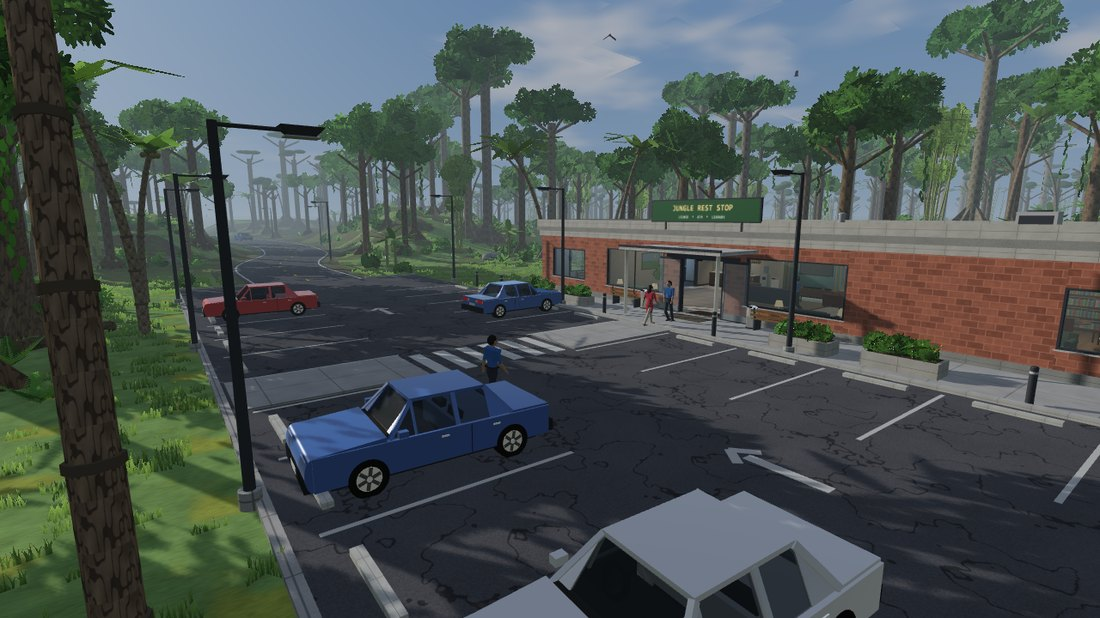
\includegraphics[width=\linewidth]{parking_lot}\caption{Parked cars and a visitor walking to the entrance}\end{subfigure}
\begin{subfigure}{0.49\linewidth}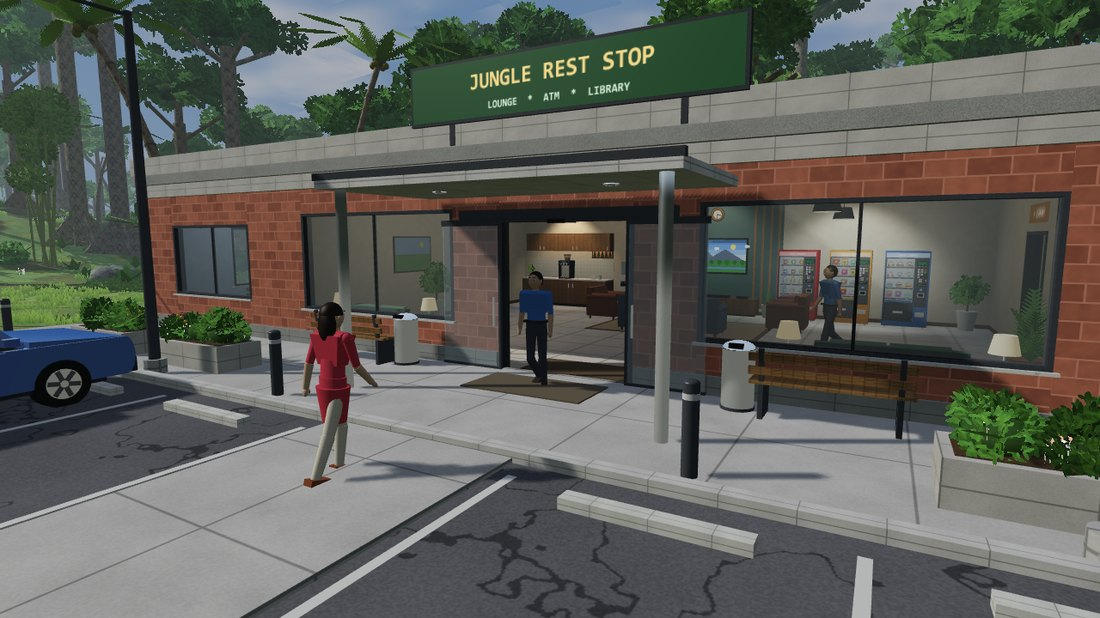
\includegraphics[width=\linewidth]{story_enter}\caption{Walking in through the sliding doors}\end{subfigure}
\begin{subfigure}{0.49\linewidth}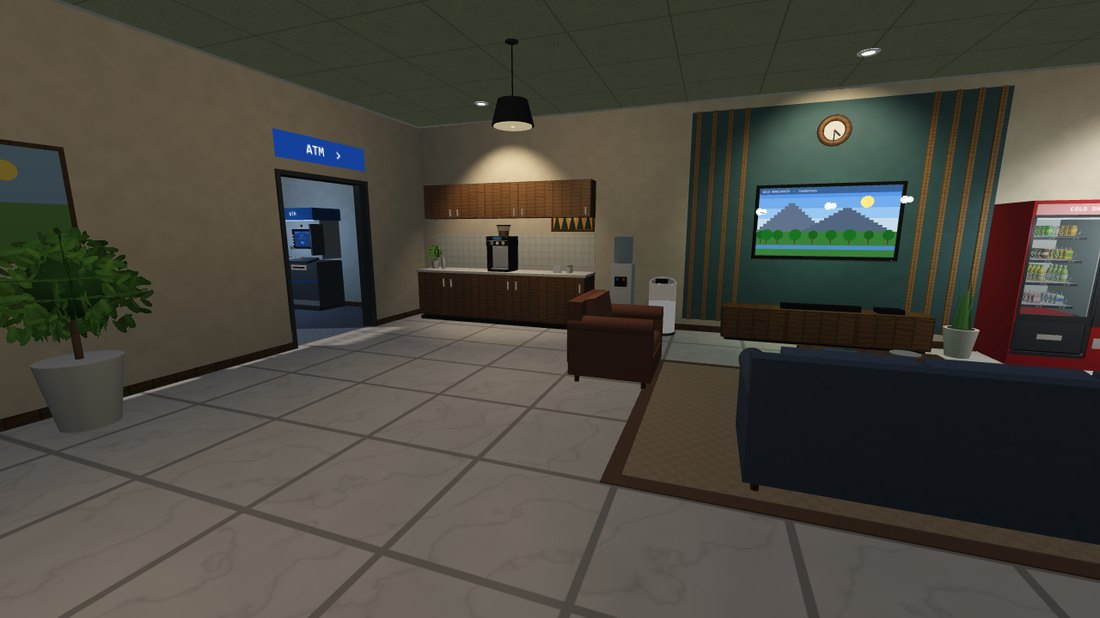
\includegraphics[width=\linewidth]{visitors_inside}\caption{Watching TV (the TV light falls on them)}\end{subfigure}
\begin{subfigure}{0.49\linewidth}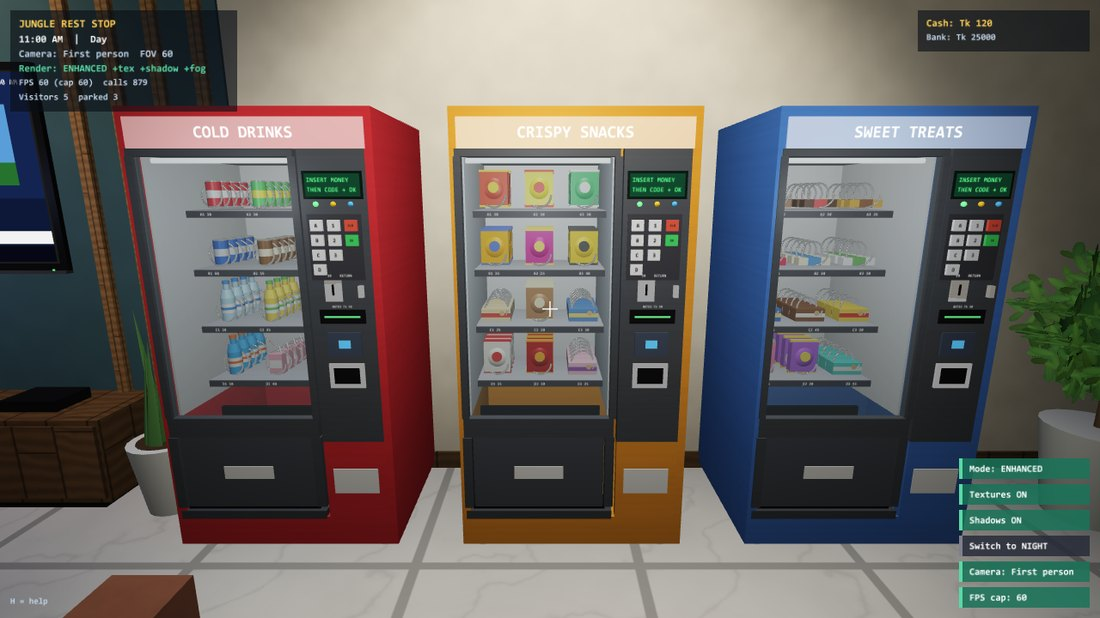
\includegraphics[width=\linewidth]{vending_row}\caption{Buying from a vending machine}\end{subfigure}
\caption{NPC visitors.}\label{fig:visitors}
\end{figure}
\Cref{lst:trace} shows the beginning of a trace recorded by the program.
\lstinputlisting[language={},caption={Start of a visitor trace (simulation time, visitor, spot, activity)},label={lst:trace},basicstyle=\ttfamily\scriptsize]{generated/visitor_trace.txt}

% =============================================================================
\section{Animation, Particles, Text and Sound}\label{sec:effects}
\subsection{Autonomous behaviour}
Every moving character is a state machine plus a simple movement rule (\Cref{tab:ai}).
\begin{table}[H]
\centering\small
\caption{Characters that move on their own}\label{tab:ai}
\begin{tabularx}{\linewidth}{@{}P{2.2cm}P{4.0cm}X@{}}
\toprule
Who & Decision (what to do) & Movement (how) \\ \midrule
Visitor & state machine with reserved resources (\Cref{fig:visitorsm}) & Dijkstra route on the waypoint graph, 1.35 m/s, waits when blocked \\
Car & part of the visitor's state machine; lot token & path following by length $s$, Bézier parking, braking limit $v\le\sqrt{2as_{left}}$ \\
Fish & swim; swim up while there is food & ellipse $x=r_x\cos\varphi$, $z=r_z\sin\varphi$, heading $\operatorname{atan2}(\Delta x,\Delta z)$ \\
Birds & fly by day & circles $\mathbf{p} = \mathbf{c} + (r\cos a,\ h + 1.5\sin 2a,\ r\sin a)$, $a \mathrel{+}= \omega\Delta t$ \\
Fireflies & appear at night, outdoors & drift on sine curves around the camera \\
\bottomrule
\end{tabularx}
\end{table}
\paragraph{Fish.} The height of a fish moves slowly towards $y_{target} = y_0 + 0.03\sin(0.7t+\varphi)$ at no more than
0.25 m/s; while there is food, $y_{target}$ is the water surface. The tail wags with $R_y(25^\circ\sin(9t+3\varphi))$.
\paragraph{Birds.} The wings are boxes in child nodes rotated by $R_z(\pm35^\circ\sin(\text{flap}))$ with
$\text{flap} \mathrel{+}= 9\,\Delta t$.
\paragraph{Fireflies.} 110 glowing spheres whose positions are wrapped into a $60\times60$ m box around the camera,
$x' = ((x - x_{cam}) \bmod 60) - 30 + x_{cam}$, so some are always near the viewer. Each blinks with
$0.5+0.5\sin(3t+3\varphi)$ and is hidden below 0.25.

\subsection{Particles}\label{sec:particles}
A particle is a small basic shape with a position $\mathbf{p}$, a velocity $\mathbf{v}$ and a life time. Every frame
$\mathbf{v} \mathrel{+}= \mathbf{g}\,\Delta t$ (for falling particles), $\mathbf{p} \mathrel{+}= \mathbf{v}\,\Delta t$ and the life decreases
by $\Delta t$; at the end of its life the particle is removed.
\begin{table}[H]
\centering\small
\caption{Particle effects}\label{tab:particles}
\begin{tabularx}{\linewidth}{@{}P{2.6cm}P{2.6cm}X@{}}
\toprule
Effect & Shape & Rule \\ \midrule
Coffee steam & transparent sphere & a new puff every 0.12 s while brewing; rises 7 cm/s and sways; grows from 2 to 6 cm; $\alpha = 0.25\cdot\text{life}$; lives 1.6 s \\
Change coins & thin cylinder & fall with $g=9.81\ \mathrm{m/s^2}$ into the coin cup \\
Falling product & the product & gravity, spin and a bounce $v_y \leftarrow -0.32\,v_y$ \\
Aquarium bubbles & transparent sphere & rise 12--22 cm/s with a wobble; restart at the bottom \\
Fish food & tiny sphere & sinks 4 cm/s, lives 5--8 s \\
Fireflies & glowing sphere & see above \\
\bottomrule
\end{tabularx}
\end{table}

\subsection{Text rendering}\label{sec:text}
All text (HUD, ATM and vending screens, TV, signs, price tags) uses one \textbf{font atlas}:
\begin{enumerate}
  \item At start-up Windows GDI draws the 95 printable ASCII characters (Consolas) into one bitmap, which becomes an
        OpenGL texture whose alpha channel is the shape of the letters.
  \item Each character is one textured quad (two triangles) whose texture coordinates select its cell in the atlas.
  \item \textbf{HUD text} uses the orthographic projection $\text{ortho}(0,W,H,0)$, so one unit is one pixel; depth
        testing is off, so it is always on top.
  \item \textbf{Text in the 3D world} is drawn on a \emph{canvas}: a flat rectangle with its own model matrix (for
        example the ATM screen). A canvas point $(x,y)$ is placed with
        $\mathbf{p} = M_{canvas}\,(x-\tfrac{w}{2},\ y-\tfrac{h}{2},\ 0,\ 1)^T$, so the text sits on the screen and turns
        with the machine. Depth testing is on, so a person in front hides the text.
\end{enumerate}
Text is blended with $C = \alpha\,C_{text} + (1-\alpha)\,C_{behind}$, which gives smooth letter edges.

\subsection{Sound}\label{sec:sound}
The sound uses 14 short recordings that are free to use (CC0, public domain; from Kenney.nl and OpenGameArt, listed
in \texttt{assets/sounds/CREDITS.txt}), stored as 44.1 kHz mono WAV files. The two background sounds (birds by day,
crickets at night) are loops whose end is cross-faded into their start. A mixer thread adds all playing sounds,
limits the sum with $\tanh$ and sends blocks of 2048 samples to the sound card with the Windows \texttt{waveOut}
functions. Sounds in the world become quieter with the distance $d$ from the camera,
\[
volume = \frac{v_0}{1+(d/4)^2},
\]
so a machine used by a visitor in another room is heard only faintly. The background is quieter inside the building.
\begin{table}[H]
\centering\small
\caption{Sounds}\label{tab:sounds}
\begin{tabularx}{\linewidth}{@{}P{3.0cm}X@{}}
\toprule
Sound & When \\ \midrule
click, beep & any button or switch; ATM keys; coffee ready \\
coin, thud, motor & vending: money in, change falling, product hitting the tray, spiral turning \\
cash, grinder, pouring & ATM gives money; coffee machine grinds and pours \\
door whoosh, car door & entrance doors start to move; a visitor opens or closes the car door \\
birds / crickets & quiet background loop by day / by night \\
\bottomrule
\end{tabularx}
\end{table}

% =============================================================================
\section{Performance}
\begin{itemize}
  \item \textbf{Instanced drawing}: all copies of one basic shape are drawn with one \texttt{glDrawElementsInstanced}
        call; each instance carries its model matrix, normal matrix, colour, emission, texture layer and material values.
  \item \textbf{Static world in chunks}: \statStaticInstances\ shapes that never move are collected once (in
        \statBuildSeconds\ s) into \statChunks\ chunks of $32\times32$ m, each with its own GPU buffer.
  \item \textbf{Culling}: a chunk is skipped when its bounding box is outside the view frustum (six planes taken from
        the view-projection matrix) or farther than 165 m. Grass and flowers end at 45 m, bushes, ferns and leaf cards at 85 m.
  \item \textbf{Occlusion culling}: visible chunks are drawn from near to far, and a chunk that was completely hidden in the
        previous frame (for example the jungle behind a wall) is skipped; only its bounding box is tested again with an
        occlusion query.
  \item \textbf{Depth pre-pass}: depth is written first with a minimal shader, then the lighting shader runs with
        \texttt{GL\_LEQUAL}, so every pixel is lit exactly once.
  \item \textbf{Per-room light lists}, frustum culling of lights, and a shadow pass that skips grass and glass.
  \item \textbf{Frame cap}: after each frame the program sleeps until $1/cap - 1.5$ ms and then waits the remaining time,
        which gives a steady 60 or 30 FPS.
\end{itemize}
\begin{table}[H]
\centering\small
\caption{Measured frame time without the frame cap (1280$\times$720, Intel Iris Xe)}
\begin{tabular}{l r r r r r}
\toprule
View & \multicolumn{2}{c}{Enhanced} & \multicolumn{2}{c}{Basic} & Triangles \\
 & ms & FPS & ms & FPS & (enh.) \\
\midrule
Outside, day & 14.0 & 72 & 10.8 & 93 & 2.25M \\
Main lounge & 11.7 & 86 & 8.3 & 120 & 2.25M \\
Inside the jungle & 10.2 & 98 & 8.3 & 121 & 1.87M \\
Parking lot, night & 11.7 & 86 & 11.2 & 90 & 1.64M \\
Aerial view & 15.3 & 66 & 12.9 & 78 & 2.16M \\
\bottomrule
\end{tabular}

\end{table}

% =============================================================================
\section{Conclusion}
Jungle Rest Stop is a small living world: three connected rooms with working machines, visitors who arrive by car and
act on their own, a dense jungle, and light that changes from morning to night. Every object is a set of basic shapes
placed with translation, rotation and scaling and organised in parent and child nodes. The project covers the main
topics of the course in one program: transformations and hierarchical modelling, viewing and projection,
illumination and shading, several light types, texture mapping, shadow mapping, fog, transparency, animation,
picking, collision detection and camera control, and it runs at a steady 60 FPS on integrated graphics.

% =============================================================================
\begin{thebibliography}{9}
\bibitem{red} J. Kessenich, G. Sellers, D. Shreiner. \emph{OpenGL Programming Guide}, 9th ed., Addison-Wesley, 2016.
\bibitem{lo} J. de Vries. \emph{Learn OpenGL}, \url{https://learnopengl.com} (lighting, shadow mapping, instancing).
\bibitem{hearn} D. Hearn, M. P. Baker, W. Carithers. \emph{Computer Graphics with OpenGL}, 4th ed., Pearson, 2010.
\bibitem{rtr} T. Akenine-M\"oller, E. Haines, N. Hoffman et al. \emph{Real-Time Rendering}, 4th ed., CRC Press, 2018.
\bibitem{blinn} J. F. Blinn. Models of light reflection for computer synthesized pictures. \emph{SIGGRAPH}, 1977.
\bibitem{williams} L. Williams. Casting curved shadows on curved surfaces. \emph{SIGGRAPH}, 1978.
\bibitem{perlin} K. Perlin. An image synthesizer. \emph{SIGGRAPH}, 1985.
\bibitem{glfw} GLFW documentation, \url{https://www.glfw.org}; GLAD loader, \url{https://glad.dav1d.de}.
\end{thebibliography}
